\section[\thesection \  Neuronale Netze]{Neuronale Netze}\label{sec:nn}

% Frame 1
\begin{frame}{Machine Learning}
        Erkennung von Zusammenhängen in großen Datenmengen,\\ohne explizite programmierung darauf.
        \begin{itemize}
            \item Supervised Learning
        \end{itemize}

        \begin{figure}[h]
            \centering
            \def\svgwidth{0.8\columnwidth}
            
\tikzset{
    decision/.style={
        diamond,
        draw,
        text width=4em,
        text badly centered,
        inner sep=-1pt,
        node distance=8em
    },
    block/.style={
        rectangle,
        draw,
        text width=6em,
        %minimum widhth=6em,
        minimum height=3.5em,
        text centered,
        node distance=20em
    },
    arrow/.style={
        draw,
        >=latex,
        ->
    },
    textfeld/.style={
        %draw,
        text centered,
        node distance=1.5em
    }
}


\begin{tikzpicture}

    
    \node (system) [block] {Klassisches\\Programm};
    \node (system2) [block, right of=system] {ML\\Programm};

    \node [textfeld, left=of system.167] (inputs) {Daten};
    \node [textfeld, left=of system.193] (regeln) {Regeln};
    \node [textfeld, right=of system] (output) {Ausgaben};

    \node [textfeld, left=of system2.167] (inputs2) {Daten};
    \node [textfeld, left=of system2.193] (output2) {Ausgaben};
    \node [textfeld, right=of system2] (regeln2) {Regeln};
    
    \draw[arrow] (inputs) -- (system.167);
    \draw[arrow] (regeln) -- (system.193);
    \draw[arrow] (system) -- (output);
    
    \draw[arrow] (inputs2) -- (system2.167);
    \draw[arrow] (output2) -- (system2.193);
    \draw[arrow] (system2) -- (regeln2);
    

\end{tikzpicture}

        \end{figure}

        \visible<2->{
        \begin{columns}[T]
        \column{0.3\columnwidth}
        \begin{block}{Neuronale Netze}

        \vspace{0.5cm}
            Für komplexere Input Daten, z.B. Bilder

    \end{block}

    \column{0.65\columnwidth}

    \begin{figure}[h]
        \centering
        \def\svgwidth{\columnwidth}
        \begin{neuralnetwork}[height=1]
    \newcommand{\nodetextclear}[2]{}
    \newcommand{\nodetexth}[2]{$h_#2$}
    \newcommand{\nodetextx}[2]{$x_#2$}
    \newcommand{\nodetexty}[2]{$y_#2$}
    \inputlayer[count=3, bias=false, title=Input\\layer, text=\nodetextx]
    \hiddenlayer[count=4, bias=false, title=Hidden\\layer, text=\nodetexth] \linklayers
    \outputlayer[count=2, title=Output\\layer, text=\nodetexty] \linklayers
\end{neuralnetwork}
    \end{figure}
    \end{columns}
        }
\end{frame}

% Frame 2
\begin{frame}{Training \& Inferenz}
    \begin{columns}[T]
        \column{0.6\columnwidth}
        Training
        \begin{figure}
            \centering
            \def\svgwidth{0.8\columnwidth}
            
\tikzstyle{process} = [rectangle, fill=blue!20, minimum width=2.5cm, minimum height=1cm, text centered, draw=black]
\tikzstyle{arrow} = [thick,->,>=stealth]

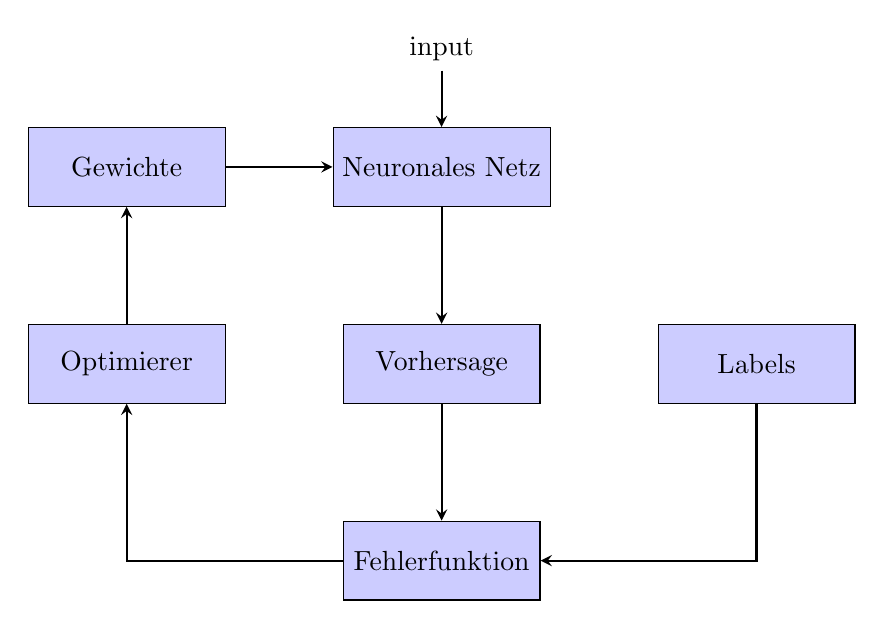
\begin{tikzpicture}[node distance=1.6cm]

  \begin{scope}[node distance=2.5cm]
    \node (nn)      [process]                   {Neuronales Netz};
    \node (pred)      [process, below of=nn]      {Vorhersage};
    \node (loss)      [process, below of=pred]      {Fehlerfunktion};
    
  \end{scope}
  
  \begin{scope}[node distance=4cm]
    \node (opt) [process, left of=pred]      {Optimierer};
    \node (weights)  [process, left of=nn] {Gewichte};
    \node (labels)   [process, right of=pred]  {Labels};
  \end{scope}

  \node (input) at (0,1.5) {input};

  \draw[arrow] (input) -- (nn);

  \draw[arrow] (nn) -- (pred);
  \draw[arrow] (pred) -- (loss);

  \draw[arrow] (labels) |- (loss);
  \draw[arrow] (loss) -| (opt);

  \draw[arrow] (opt) -- (weights);
  \draw[arrow] (weights) -- (nn);
  
    
\end{tikzpicture}

        \end{figure}
        \begin{itemize}
            \item variable Parameter: \textit{Weights}
            \item bekannte Input Daten: \textit{Labels}
            \item mehrfaches durchlaufen: \textit{Epochen}
        \end{itemize}
        \column{0.4\columnwidth}
        \visible<2->{
        Inferenz
        \begin{figure}
            \centering
            \def\svgwidth{0.4\columnwidth}
            \input{Bilder/infer_workflow.pdf_tex}
        \end{figure}
        \begin{itemize}
            \item fixe Parameter
            \item unbekannte Input Daten
            \item einmaliges durchlaufen
        \end{itemize}
        }
    \end{columns}
\end{frame}


